\documentclass[twocolumn]{article}
\usepackage[fontsize=12pt]{scrextend}
\usepackage{float}

% COLORS %

\usepackage{xcolor}
\definecolor{bg}{RGB}{22,43,58}
\definecolor{bgTitle}{RGB}{52,75,85}
\definecolor{fgTitle}{RGB}{230,230,230}
\definecolor{linkColor}{RGB}{2,11,120}

% CODE BLOCKS STYLING %

\usepackage[T1]{fontenc}
\usepackage[ttdefault=true]{AnonymousPro}
\usepackage{listings}
\usepackage{minted}
\usepackage{tcolorbox}
\tcbuselibrary{listings, breakable, minted, skins}
\tcbset{listing engine=minted}

\newtcblisting{javaCode}[2][]{
    breakable,
    listing only, #1 ,title=#2,
    minted language=java,
    minted style=monokai,
    coltitle=fgTitle,
    colbacktitle=bgTitle,
    toptitle=3mm, bottomtitle=2.5mm,
    top=2mm, bottom=3mm,
    fonttitle=\footnotesize\ttfamily,
    colback=bg, enhanced, frame hidden, 
    minted options={fontfamily=AnonymousPro, 
    tabsize=4, breaklines, autogobble, fontsize=\scriptsize}
}
    
\newtcblisting{yamlCode}[2][]{
    breakable,
    listing only, #1 ,title=#2,
    minted language=yaml,
    minted style=friendly,
    coltitle=fgTitle,
    colbacktitle=bgTitle,
    toptitle=3mm, bottomtitle=2.5mm,
    top=2mm, bottom=3mm,
    fonttitle=\normalsize\ttfamily,
    enhanced, frame hidden, 
    minted options={fontfamily=AnonymousPro, 
    tabsize=4, breaklines, autogobble, linenos=false, fontsize=\scriptsize}
}

\setminted[java]{fontfamily=AnonymousPro, fontsize=\footnotesize, breaksymbol=.}
\setminted[yaml]{fontfamily=AnonymousPro, fontsize=\footnotesize, breaksymbol=}

% DOCUMENT SETUP %

\usepackage[italian]{babel}
\usepackage[a4paper,top=2.5cm,bottom=2.5cm,left=3cm,right=3cm,marginparwidth=1.75cm,footskip=1.25cm,heightrounded]{geometry}

\usepackage{amsmath}
\usepackage{graphicx}
\usepackage[colorlinks=true, allcolors=linkColor]{hyperref}
\usepackage{wrapfig}

\graphicspath{ {./images/} }
\usepackage{subfig}

\usepackage{tgschola}
\linespread{1.5}

\title{Relazione su Applicativo Java\newline per la Gestione del Diabete}
\author{Federico Marra - Alberto del Buono Paolini}
\date{Ottobre - Dicembre 2023}

\begin{document}

% INITIAL PAGE %

\begin{onecolumn}
\maketitle
\thispagestyle{empty}
\vspace{2em}
\begin{center}
    
\includegraphics[width=5cm]{unifi_v.png}\\[1cm]
    \textsc{\Large Dipartimento di Ingegneria dell'Informazione}\\[0.25cm]
    \textsc{\Large Ingegneria del Software}\\
    \vspace{2.5em}
    \href{https://github.com/federicomarra/swe-diab}{
        \raisebox{-.3\height}{
\includegraphics[width=1.2cm]{images/github-logo.png}}
        \hspace{.3em}
        \Large{Repository Github}
    }
\end{center}
\end{onecolumn}

% INDEX %

\begin{onecolumn}
\tableofcontents    % Indice
\thispagestyle{empty}
\vspace{1cm}
\setcounter{page}{1}
\end{onecolumn}
%\pagebreak
\newpage

% CONTENT %

\section{Motivazione e Descrizione}
Vogliamo modellare un sistema che controlli una \href{https://it.wikipedia.org/wiki/Microinfusore}{\textit{patch-pump}} (detto anche microinfusore), quindi per la gestione insulinica, questo svolge due funzioni principali:
\begin{enumerate}
    \item \textbf{Bolo}: È un bolo calcolato da una glicemia e una massa di carboidrati data in input dall'utente e divisi per fattori che dipendono dall'orario corrente, ci sono diverse opzioni tenendo per esempio conto dei vecchi boli e del decadimento lineare dell'insulina ancora attiva.
    \item \textbf{Basale}: Fornisce una base continua di insulina erogata con una certa frequenza.
\end{enumerate}
Modellizzando, queste funzioni vengono controllate tramite un palmare (Handheld Tracker) connesso via bluetooth alla patch installata sull'utente (Glucose Delivery System).
Dal palmare è possibile creare un nuovo bolo in quattro modalità o modificare uno dei tre profili orari che viene salvata in un database locale, di cui può essere eseguito un backup su un database cloud (gestito da Cloud Interface).
Quando si crea un bolo viene anche inviato al Glucose Delivery System che provvederà a controllare l'autenticità della richiesta ed erogarlo.
L'utente può anche modificare il valore dell'insulina basale per certe ore, questo viene salvato nel profilo basale (Basal Profile) e conservato nel database locale.
Il sistema a patch che consideriamo comprende anche una modalità di utilizzo standalone (senza palmare), infatti il Glucose Delivery System ha la possibilità di erogare automaticamente un bolo in base ai valori di glicemia letti dal suo stesso sensore, senza comunicare col palmare.

\subsection{Possibili aggiunte}
Nonostante siano state implementate solo in parte, riportiamo di seguito dei possibili sviluppi ulteriori per il nostro applicativo:

\begin{enumerate}
    \setlength\itemsep{0em}
    \item \textbf{Dashboard Web}
    \item \textbf{Routine Insulina Basale}
    \item \textbf{Routine Bolo Automatico}
\end{enumerate}

\subsubsection{Dashboard Web}

Un'interfaccia grafica accessibile dal web (analoga alla GUI già implementata per i vari client) che include grafici e tabelle aggiuntivi. L'implementazione di questa funzionalità richiede un secondo server per ospitare la dashboard che dovrebbe includere un layer di autenticazione (permettendo ad un utente di controllare solo la sua pompa di insulina).

\vspace{0.75em}
\begin{figure}[H]
    \centering
    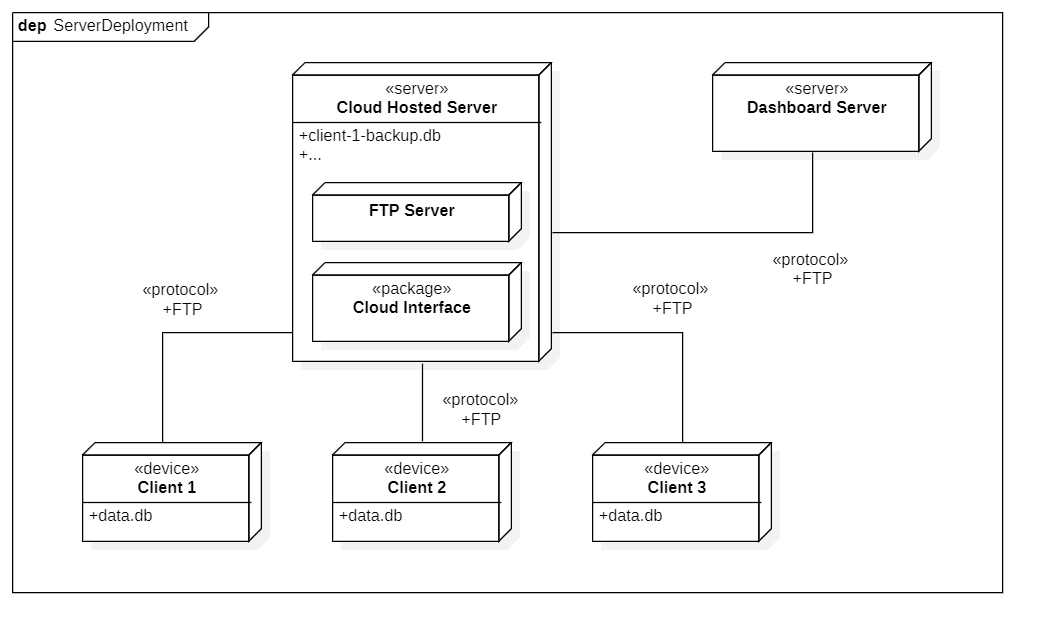
\includegraphics[width=14cm]{images/ServerDeployment.png}
    \caption{Deployment Diagram}
    \label{fig:deployment}
\end{figure}

\subsubsection{Routine Insulina Basale}

Una routine che attraverso un thread ogni 10/15 minuti inietti il quantitativo di insulina basale in percentuale alla frequenza (ad esempio: 10 min \(\rightarrow \frac{1}{6}\)), 15 min \(\rightarrow \frac{1}{4}\)) che è contenuto nel profilo orario.

\subsubsection{Routine Bolo Automatico}
Una routine che attraverso un thread ogni 10/15 minuti, prenda la glicemia dal sensore, controlli che non sia sopra una certa soglia (di solito 180mg/dL) e che se lo è esegue un bolo correttivo sottraendoci però l'insulina che è attiva.

\newpage
\section{Requisiti}

\subsection{Use Case}
Dalla descrizione del nostro modello di dominio abbiamo identificato gli use cases che può incontrare l'utente. Di seguito viene riportato l’Use Case Diagram risultante:

\null\vfill
\begin{figure}[!htbp]
    \centering
    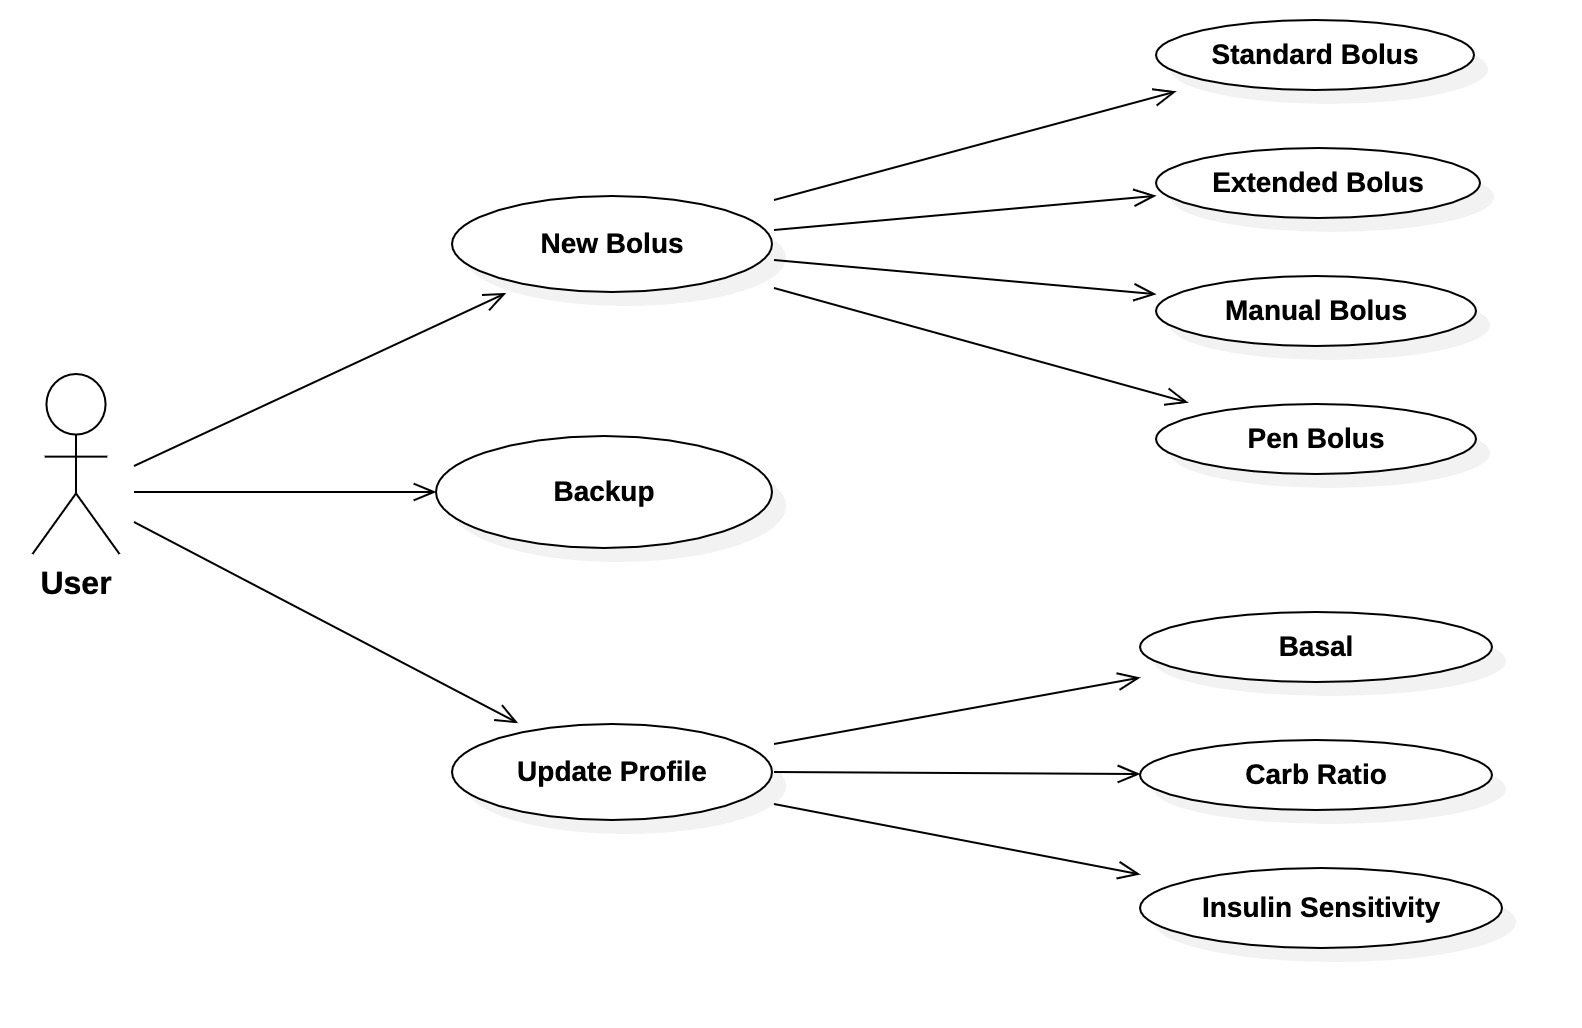
\includegraphics[width=14cm]{UseCaseDiagram.jpg}
    \caption{Use Case Diagram}
    \label{fig:use-case}
\end{figure}
\vfill\null

\newpage
\subsection{Use Case Template}

Riportiamo di seguito i template relativi a tutti i casi d’uso individuati nel nostro progetto.

\null\vfill
\begin{table}[!htbp]
\centering
\captionsetup{justification=centering}
\begin{tabular}{|p{4.5cm}|p{9.5cm}|}
    \hline
    Use Case 1 & Bolo Standard - Standard Bolus\\
    \hline
    Livello & User Goal \\
    \hline
    Descrizione & L'utente immette la quantità di carboidrati e il sistema esegue il bolo d'insulina.\\
    \hline
    Attori & User \\
    \hline
    Pre-condizioni & Nessuna\\
    \hline
    Post-condizioni & Viene inviata la quantità di unità calcolata alla Pump se tale quantità è $> 0$.\\
    \hline
    Normale svolgimento & Viene letta l'ultima glicemia, se è di più di 10 minuti fa viene effettuata una nuova misurazione, viene preso il valore dei carboidrati e dell'insulina attiva. Con tutto ciò si calcola l'insulina che il sistema inietterà.\\
    \hline
    Svolgimenti alternativi & Se i carboidrati sono 0, verranno calcolatate solo le unità per correggere se la glicemia è oltre una certa soglia \\
    \hline
\end{tabular}
\caption{Use Case Template 1 che consiste nel richiedere al sistema il calcolo delle unità e l'iniezione immediata di insulina in modalità standard.}
\label{tab:uc1}
\end{table}
\vfill\null

\begin{table}
    \centering
    \captionsetup{justification=centering}
    \begin{tabular}{|p{4.5cm}|p{9.5cm}|}
        \hline
        Use Case 2 & Bolo Esteso - Extended Bolus\\
        \hline
        Livello & User Goal \\
        \hline
        Descrizione & L'utente immette la quantità di carboidrati e quanti minuti aspettare, e il sistema esegue il bolo d'insulina.\\
        \hline
        Attori & User \\
        \hline
        Pre-condizioni & Nessuna\\
        \hline
        Post-condizioni & Viene inviata la quantità di unità dopo un numero di minuti corrispondenti al \texttt{delay} \\
        \hline
        Normale svolgimento & Simile all'UC1 ma con in aggiunta in input di quanti minuti viene ritardata l'iniezione.\\
        \hline
        Svolgimenti alternativi & Come UC1, se i carboidrati sono 0, verranno calcolatate solo le unità per correggere se la glicemia è oltre una certa soglia \\
        \hline
    \end{tabular}
    \caption{Use Case Template 2 che consiste nel richiedere al sistema il calcolo delle unità e l'iniezione di insulina in modalità estesa.}
    \label{tab:uc2}
\end{table}

\begin{table}
    \centering
    \captionsetup{justification=centering}
    \begin{tabular}{|p{4.5cm}|p{9.5cm}|}
        \hline
        Use Case 3 & Quante unità? - How Many Units?\\
        \hline
        Livello & User Goal \\
        \hline
        Descrizione & L'utente immette i carboidrati e riceve in output quante unità di insulina deve eseguire manualmente\\
        \hline
        Attori & User \\
        \hline
        Pre-condizioni & Nessuna\\
        \hline
        Post-condizioni & Viene salvata la quantità di unità calcolata\\
        \hline
        Normale svolgimento & Fornisce solo il risultato del calcolo delle unità ma non inietta, indicherà invece quante unità eseguire manualmente.\\
        \hline
        Svolgimenti alternativi & Se i carboidrati sono 0, verranno calcolate solo le unità per correggere se la glicemia è oltre una certa soglia\\
        \hline
    \end{tabular}
    \caption{Use Case Template 3 che consiste nel richiedere al sistema il calcolo delle unità e l'iniezione di insulina in modalità manuale.}
    \label{tab:uc3}
\end{table}

\begin{table}
    \centering
    \captionsetup{justification=centering}
    \begin{tabular}{|p{4.5cm}|p{9.5cm}|}
        \hline
        Use Case 4 & Bolo Penna - Pen Bolus\\
        \hline
        Livello & User Goal \\
        \hline
        Descrizione & Si inserisce nel sistema quante unità sono state fatte manualmente\\
        \hline
        Attori & User \\
        \hline
        Pre-condizioni & Si deve aver già eseguito manualmente un'iniezione di insulina\\
        \hline
        Post-condizioni & È utile per altri boli eseguiti nelle 3 ore successivi\\
        \hline
        Normale svolgimento & Viene chiesto il numero di unità iniettate, di conseguenza viene salvato nel database il bolo con le unità prese in input e con orario l'ora di immissione\\
        \hline
        Svolgimenti alternativi & Se i carboidrati sono 0, verranno calcolate solo le unità per correggere se la glicemia è oltre una certa soglia\\
        \hline
    \end{tabular}
    \caption{Use Case Template 4 che consiste nel richiedere al sistema il calcolo delle unità da poi iniettare personalmente mediante una penna di insulina.}
    \label{tab:uc4}
\end{table}

\begin{table}
    \centering
    \captionsetup{justification=centering}
    \begin{tabular}{|p{4.5cm}|p{9.5cm}|}
        \hline
        Use Case 5 & Aggiornamento del profilo di Basale - Update basal profile\\
        \hline
        Livello & User Goal \\
        \hline
        Descrizione & Si aggiorna il profilo \texttt{Basal}, ovvero delle basali (unità di insulina basale, o di fondo o di base necessarie per un singolo orario)\\
        \hline
        Attori & User \\
        \hline
        Pre-condizioni & Dev'esserci già un profilo da aggiornare (questo viene creato quando si fa partire il sistema)\\
        \hline
        Post-condizioni & Viene modificato l'\texttt{hourlyFactor} relativo al singolo orario\\
        \hline
        Normale svolgimento & In input si passa un orario e il numero di unità con cui sovrascrivere quelle precedentemente nell'\texttt{hourlyFactor} relativo all'orario\\
        \hline
        Svolgimenti alternativi & Se viene immesso come orario 0 o 24, il funzionamento è il medesimo\\
        \hline
    \end{tabular}
    \caption{Use Case Template 5 che consiste nel richiedere al sistema l'aggiornamento del profilo orario della .}
    \label{tab:uc5}
\end{table}

\begin{table}
    \centering
    \captionsetup{justification=centering}
    \begin{tabular}{|p{4.5cm}|p{9.5cm}|}
        \hline
        Use Case 6 & Aggiornamento del profilo del rapporto insulina carboidrati - Update carb ratio profile\\
        \hline
        Livello & User Goal \\
        \hline
        Descrizione & Si aggiorna il profilo \texttt{IC}, ovvero dei rapporti insulina carboidrati (peso in grammi dei carboidrati coperto da un'unità di insulina)\\
        \hline
        Attori & User \\
        \hline
        Pre-condizioni & Dev'esserci già un profilo da aggiornare (questo viene creato quando si fa partire il sistema)\\
        \hline
        Post-condizioni & Viene modificato l'\texttt{hourlyFactor} relativo al singolo orario\\
        \hline
        Normale svolgimento & In input si passa un orario e il numero di unità con cui sovrascrivere quelle precedentemente nell'\texttt{hourlyFactor} relativo all'orario\\
        \hline
        Svolgimenti alternativi & Se viene immesso come orario 0 o 24, il funzionamento è il medesimo\\
        \hline
    \end{tabular}
    \caption{Use Case Template 6 che consiste nel richiedere al sistema l'aggiornamento del profilo orario della .}
    \label{tab:uc6}
\end{table}

\begin{table}
    \centering
    \captionsetup{justification=centering}
    \begin{tabular}{|p{4.5cm}|p{9.5cm}|}
        \hline
        Use Case 7 & Aggiornamento del profilo di sensitività di insulina - Update insulin sensitivity profile\\
        \hline
        Livello & User Goal \\
        \hline
        Descrizione & Si aggiorna il profilo \texttt{IS}, ovvero delle sensitività insuliniche (di che valore glicemico scende con un'unità di insulina)\\
        \hline
        Attori & User \\
        \hline
        Pre-condizioni & Dev'esserci già un profilo da aggiornare (questo viene creato quando si fa partire il sistema)\\
        \hline
        Post-condizioni & Viene modificato l'\texttt{hourlyFactor} relativo al singolo orario\\
        \hline
        Normale svolgimento & In input si passa un orario e il numero di unità con cui sovrascrivere quelle precedentemente nell'\texttt{hourlyFactor} relativo all'orario\\
        \hline
        Svolgimenti alternativi & Se viene immesso come orario 0 o 24, il funzionamento è il medesimo\\
        \hline
    \end{tabular}
    \caption{Use Case Template 7 che consiste nel richiedere al sistema l'aggiornamento del profilo orario della .}
    \label{tab:uc7}
\end{table}

\begin{table}[!htbp]
    \centering
    \captionsetup{justification=centering}
    \begin{tabular}{|p{4.5cm}|p{9.5cm}|}
        \hline
        Use Case 8 & Backup\\
        \hline
        Livello & User Goal \\
        \hline
        Descrizione & Viene fatto un backup del database \texttt{db/data.db} in locale nel file \texttt{db/backup.db}\\
        \hline
        Attori & User \\
        \hline
        Pre-condizioni & Deve esistere un file \texttt{db/data.db} di cui fare il backup\\
        \hline
        Post-condizioni & Viene creato o sovrascritto il database \texttt{backup.db}\\
        \hline
        Normale svolgimento & Il backup viene fatto in locale nella cartella \texttt{db}\\
        \hline
        Svolgimenti alternativi & Se viene impostato un file \texttt{.env} si può uploadare il file di backup su un server sqlite.\\
        \hline
    \end{tabular}
    \caption{Use Case Template 8 che consiste nell'eseguire una copia del database con il nome di \texttt{backup.db}.}
    \label{tab:uc8}
\end{table}

\clearpage

\subsection{Mockups}

La GUI (Interfaccia Utente Grafica) è stata implementata usando il framework \href{https://it.wikipedia.org/wiki/Swing_(Java)}{\textit{Swing}} ed è compilata in un \texttt{.jar} reperibile pubblicamente nella \href{https://github.com/federicomarra/swe-diab/releases}{\textit{Release Github}}; nell'ultimo capitolo discuteremo come il processo di packaging e distribuzione è stato automatizzato.

Riportiamo di seguito i mockups realizzati relativi alla GUI per l’interazione dell'utente con il gestore del diabete. Oltre ad agire come mockup, la GUI è funzionante in tutti i casi d'uso precedentemente elencati.

\null\vfill
\begin{figure}[!htbp]
    \centering
    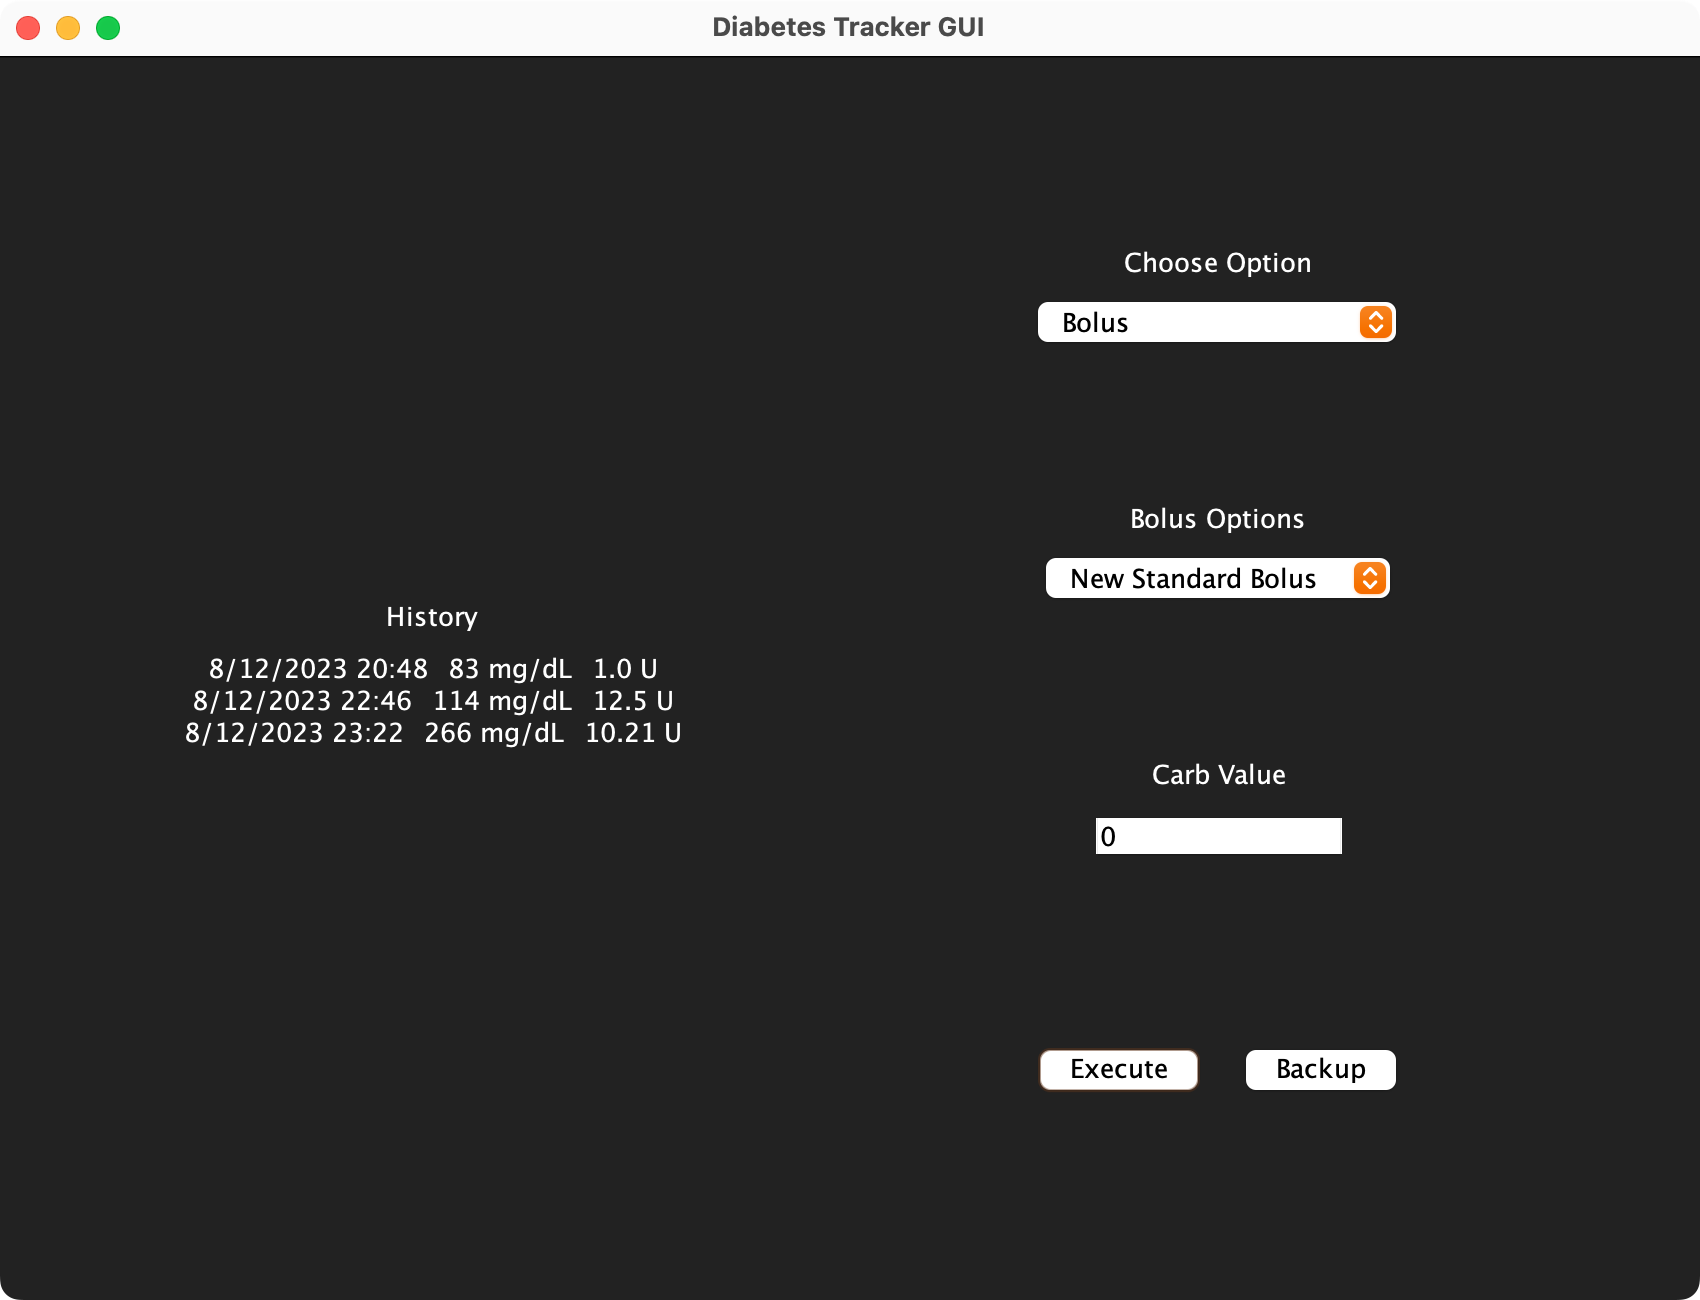
\includegraphics[width=14cm]{gui-history.png}
    \caption{Storico dei boli sulla sinistra}
    \label{fig:gui-history}
\end{figure}
\vfill\null

\begin{figure}
    \centering
    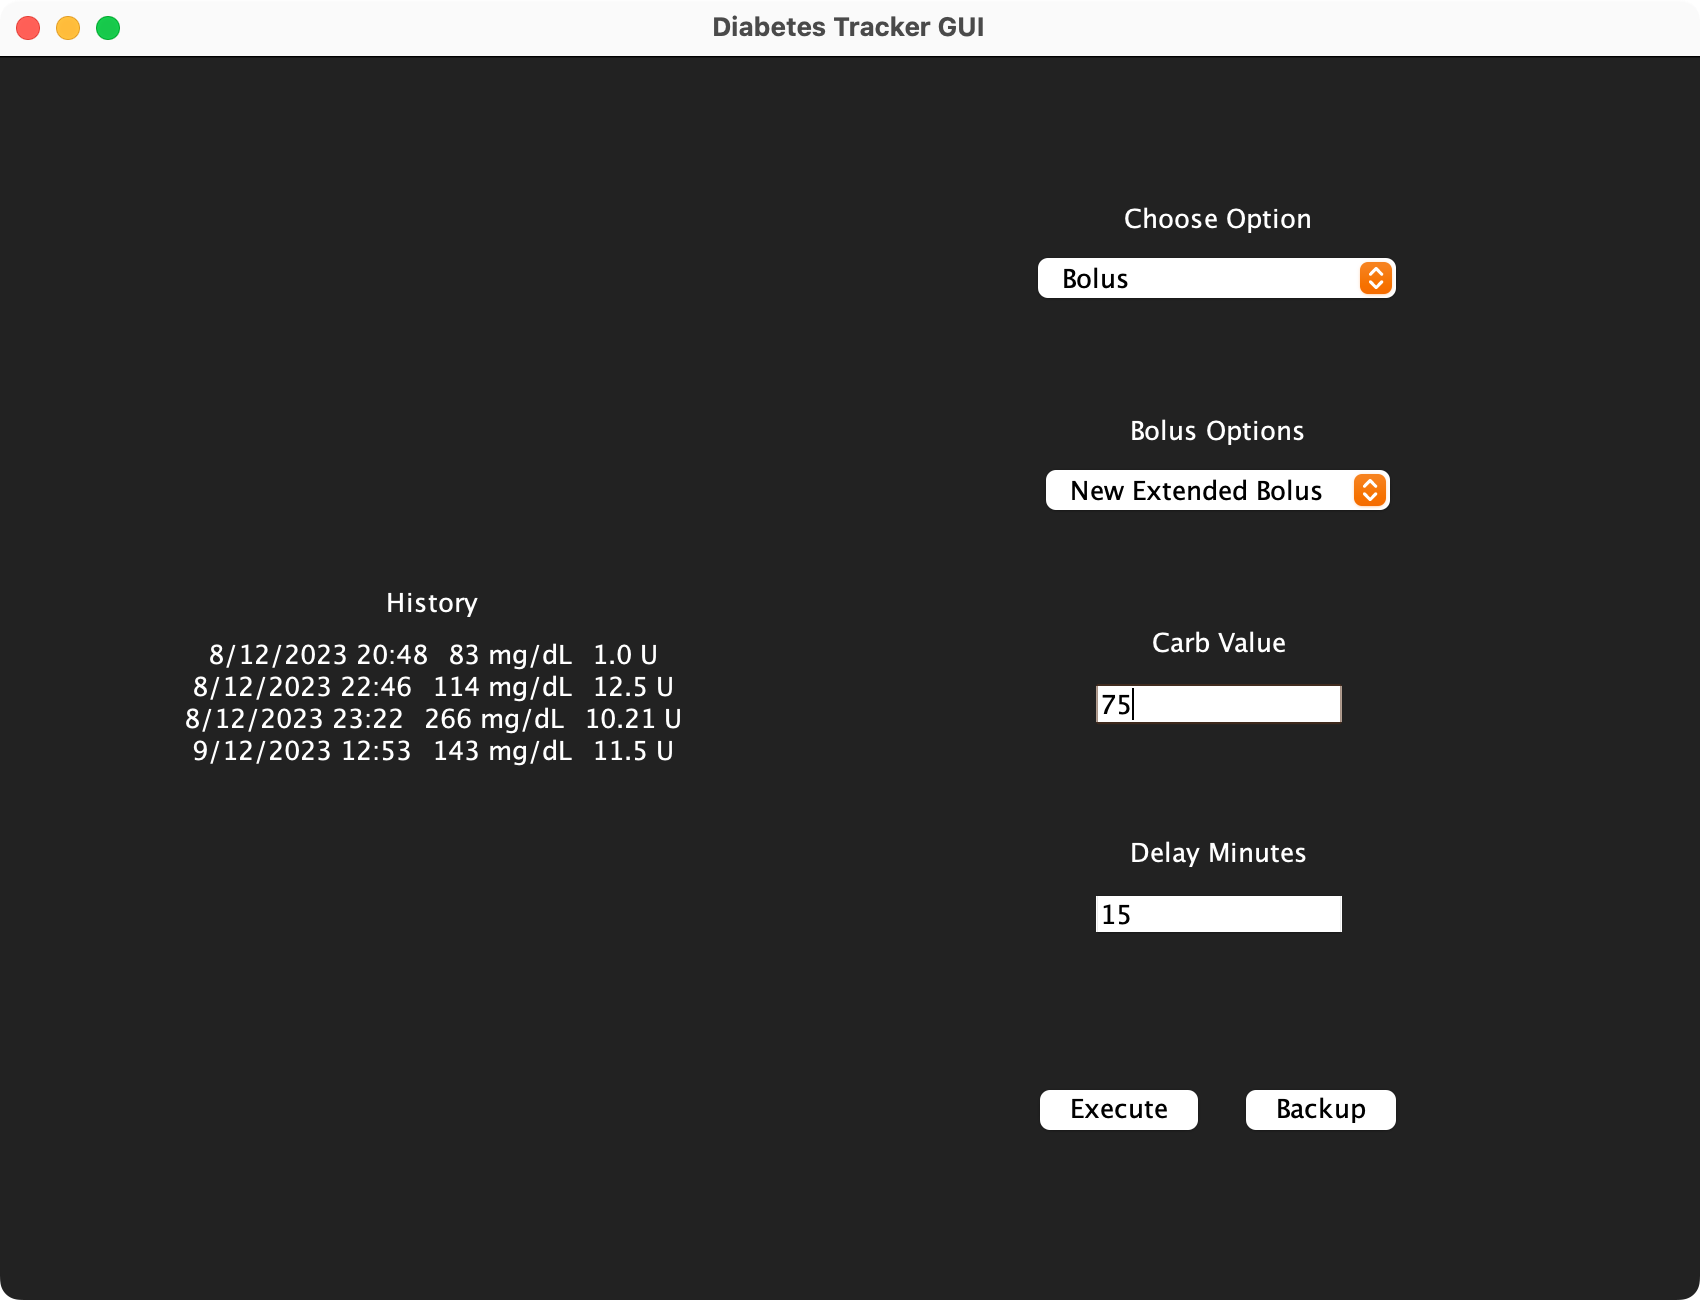
\includegraphics[width=14cm]{gui-bolus-ext.png}
    \caption{Creazione bolo in modalità estesa}
    \label{fig:gui-bolus-ext}
\end{figure}

\begin{figure}
    \centering
    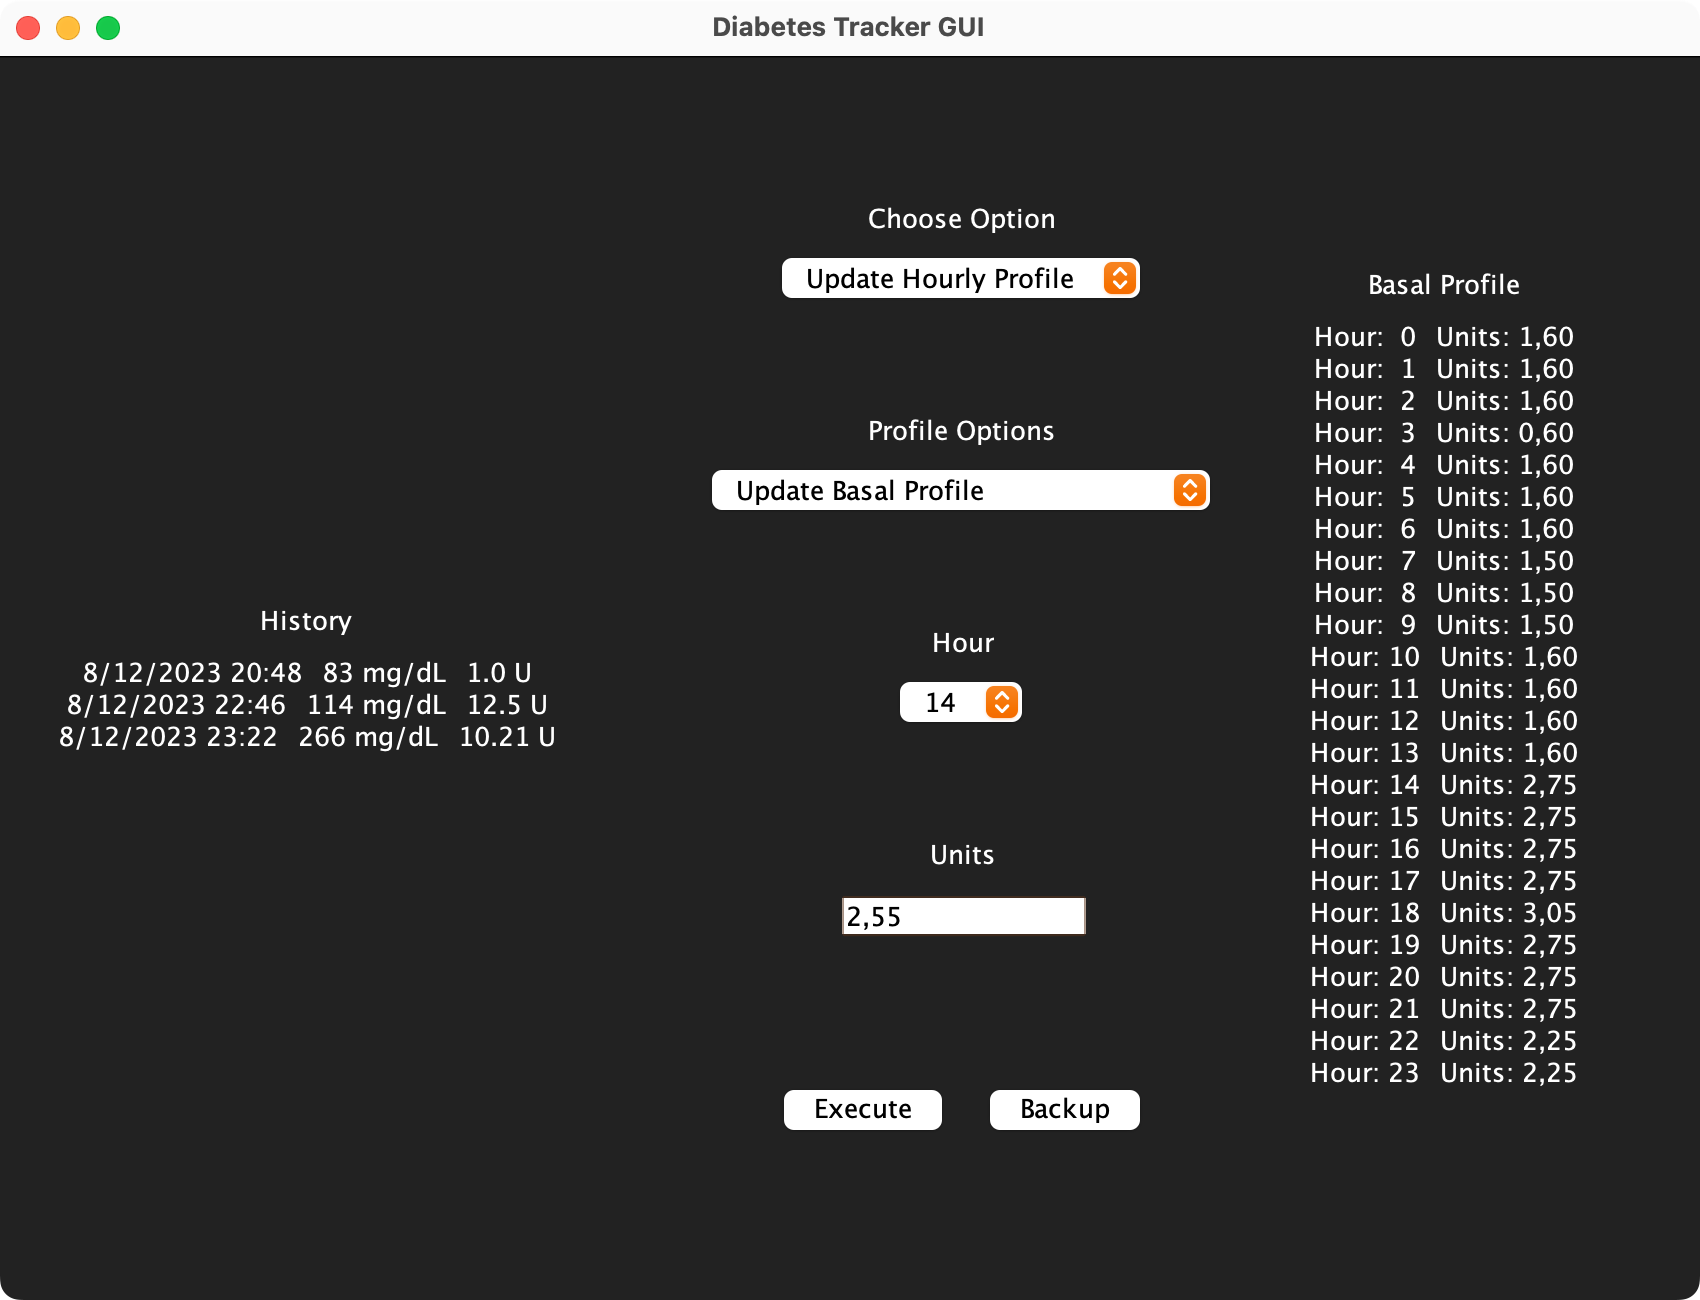
\includegraphics[width=14cm]{gui-basal.png}
    \caption{Aggiornamento profilo orario della basale}
    \label{fig:gui-basal}
\end{figure}

\begin{figure}[!htbp]
    \centering
    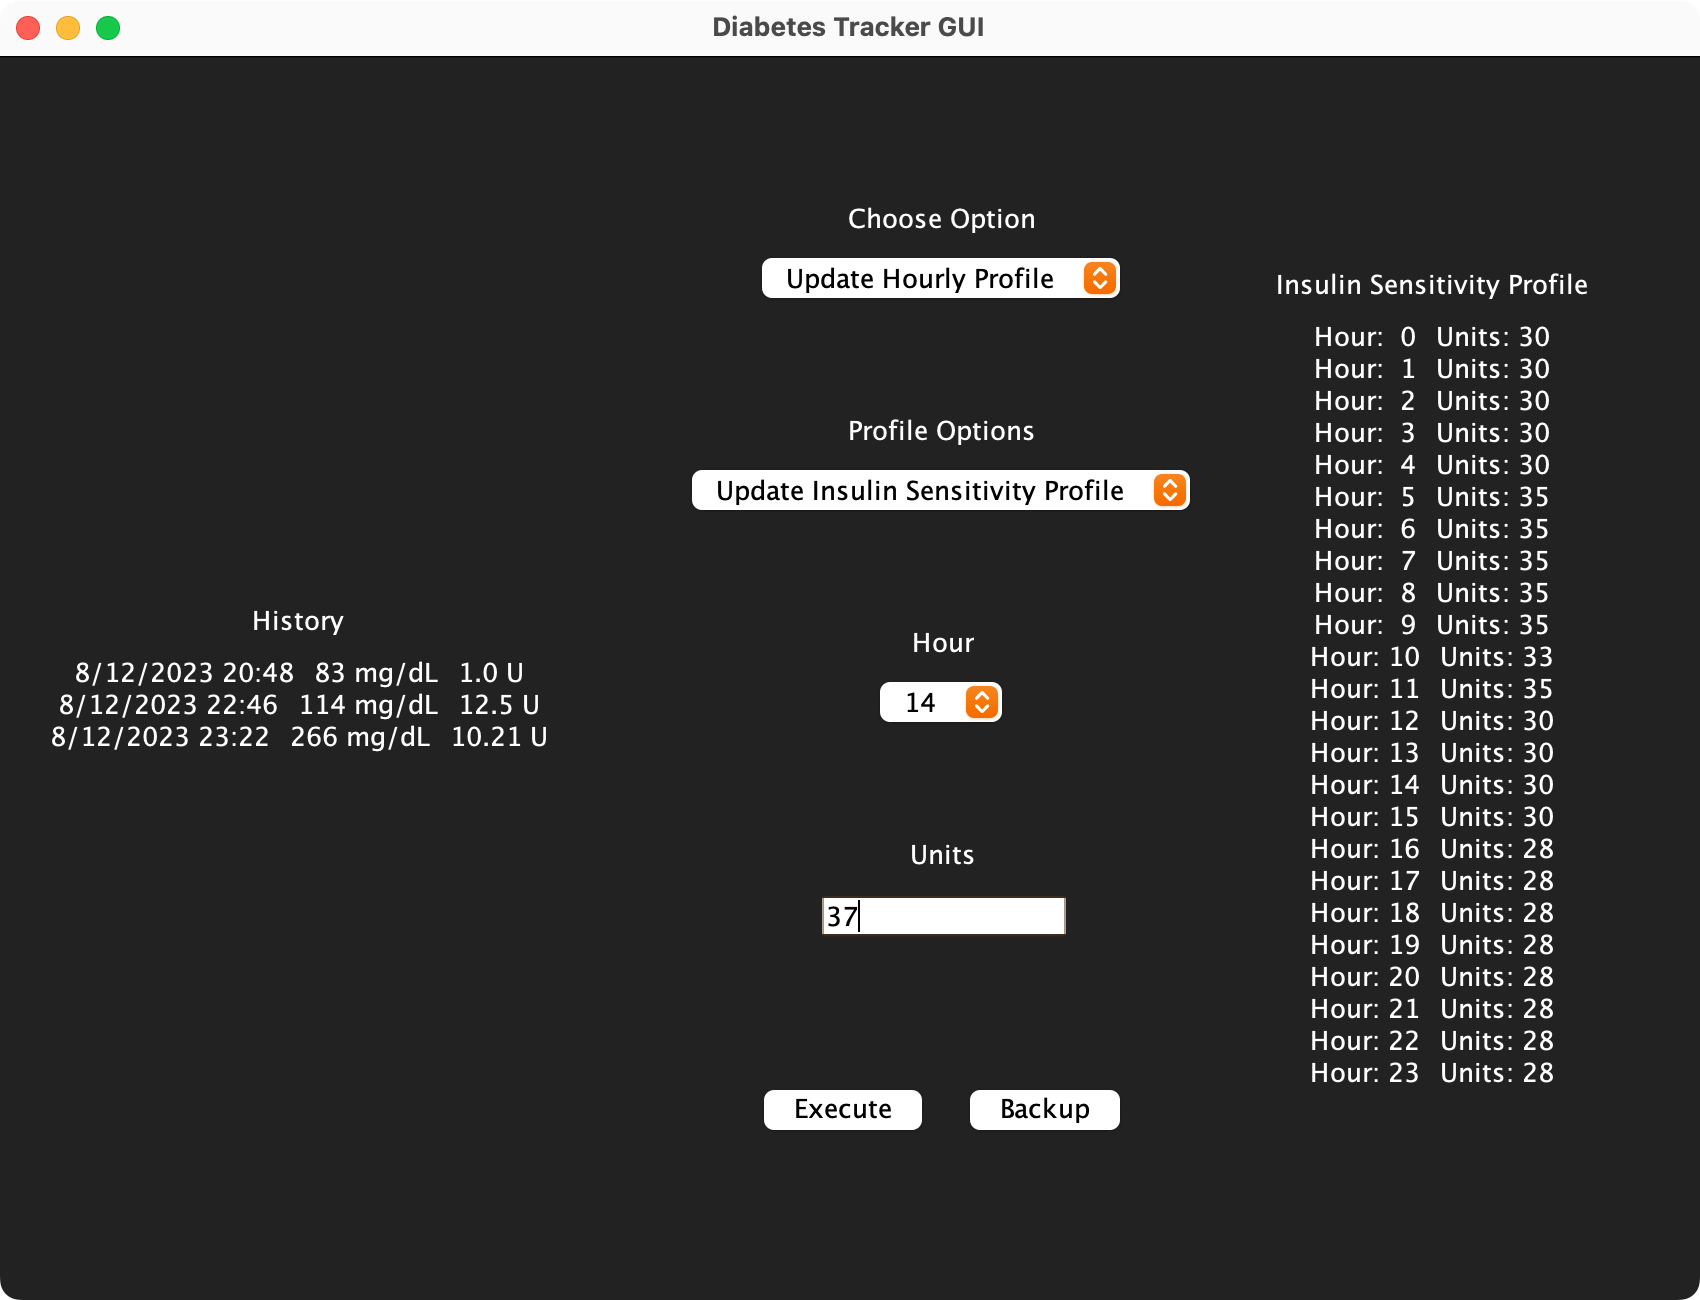
\includegraphics[width=14cm]{gui-insens.png}
    \caption{Aggiornamento profilo orario della sensitività dell'insulina}
    \label{fig:gui-insens}
\end{figure}


\section{Progettazione e Implementazione} 

\subsection{Scelte implementative e considerazioni}
Per implementare il nostro progetto in linguaggio Java ed eseguire i test ci siamo serviti delle IDE \href{https://www.jetbrains.com/idea/}{\textit{IntelliJIdea}} e \href{https://code.visualstudio.com/}{\textit{Visual Studio Code}}. Al fine di semplificare la collaborazione abbiamo utilizzato \href{https://github.com/federicomarra/swe-diab}{GitHub} come stumento di versionamento del codice. Per quanto riguarda il Class Diagram, l’Use Case Diagram e lo schema architetturale in packages ci siamo serviti del software \href{https://staruml.io/}{\textit{StarUML}}.

\subsection{Class Diagram}

Qui di seguito riportiamo la realizzazione del class diagram che descrive la nostra logica di dominio in prospettiva di implementazione:
\clearpage
\begin{figure}[H]
    \centering
    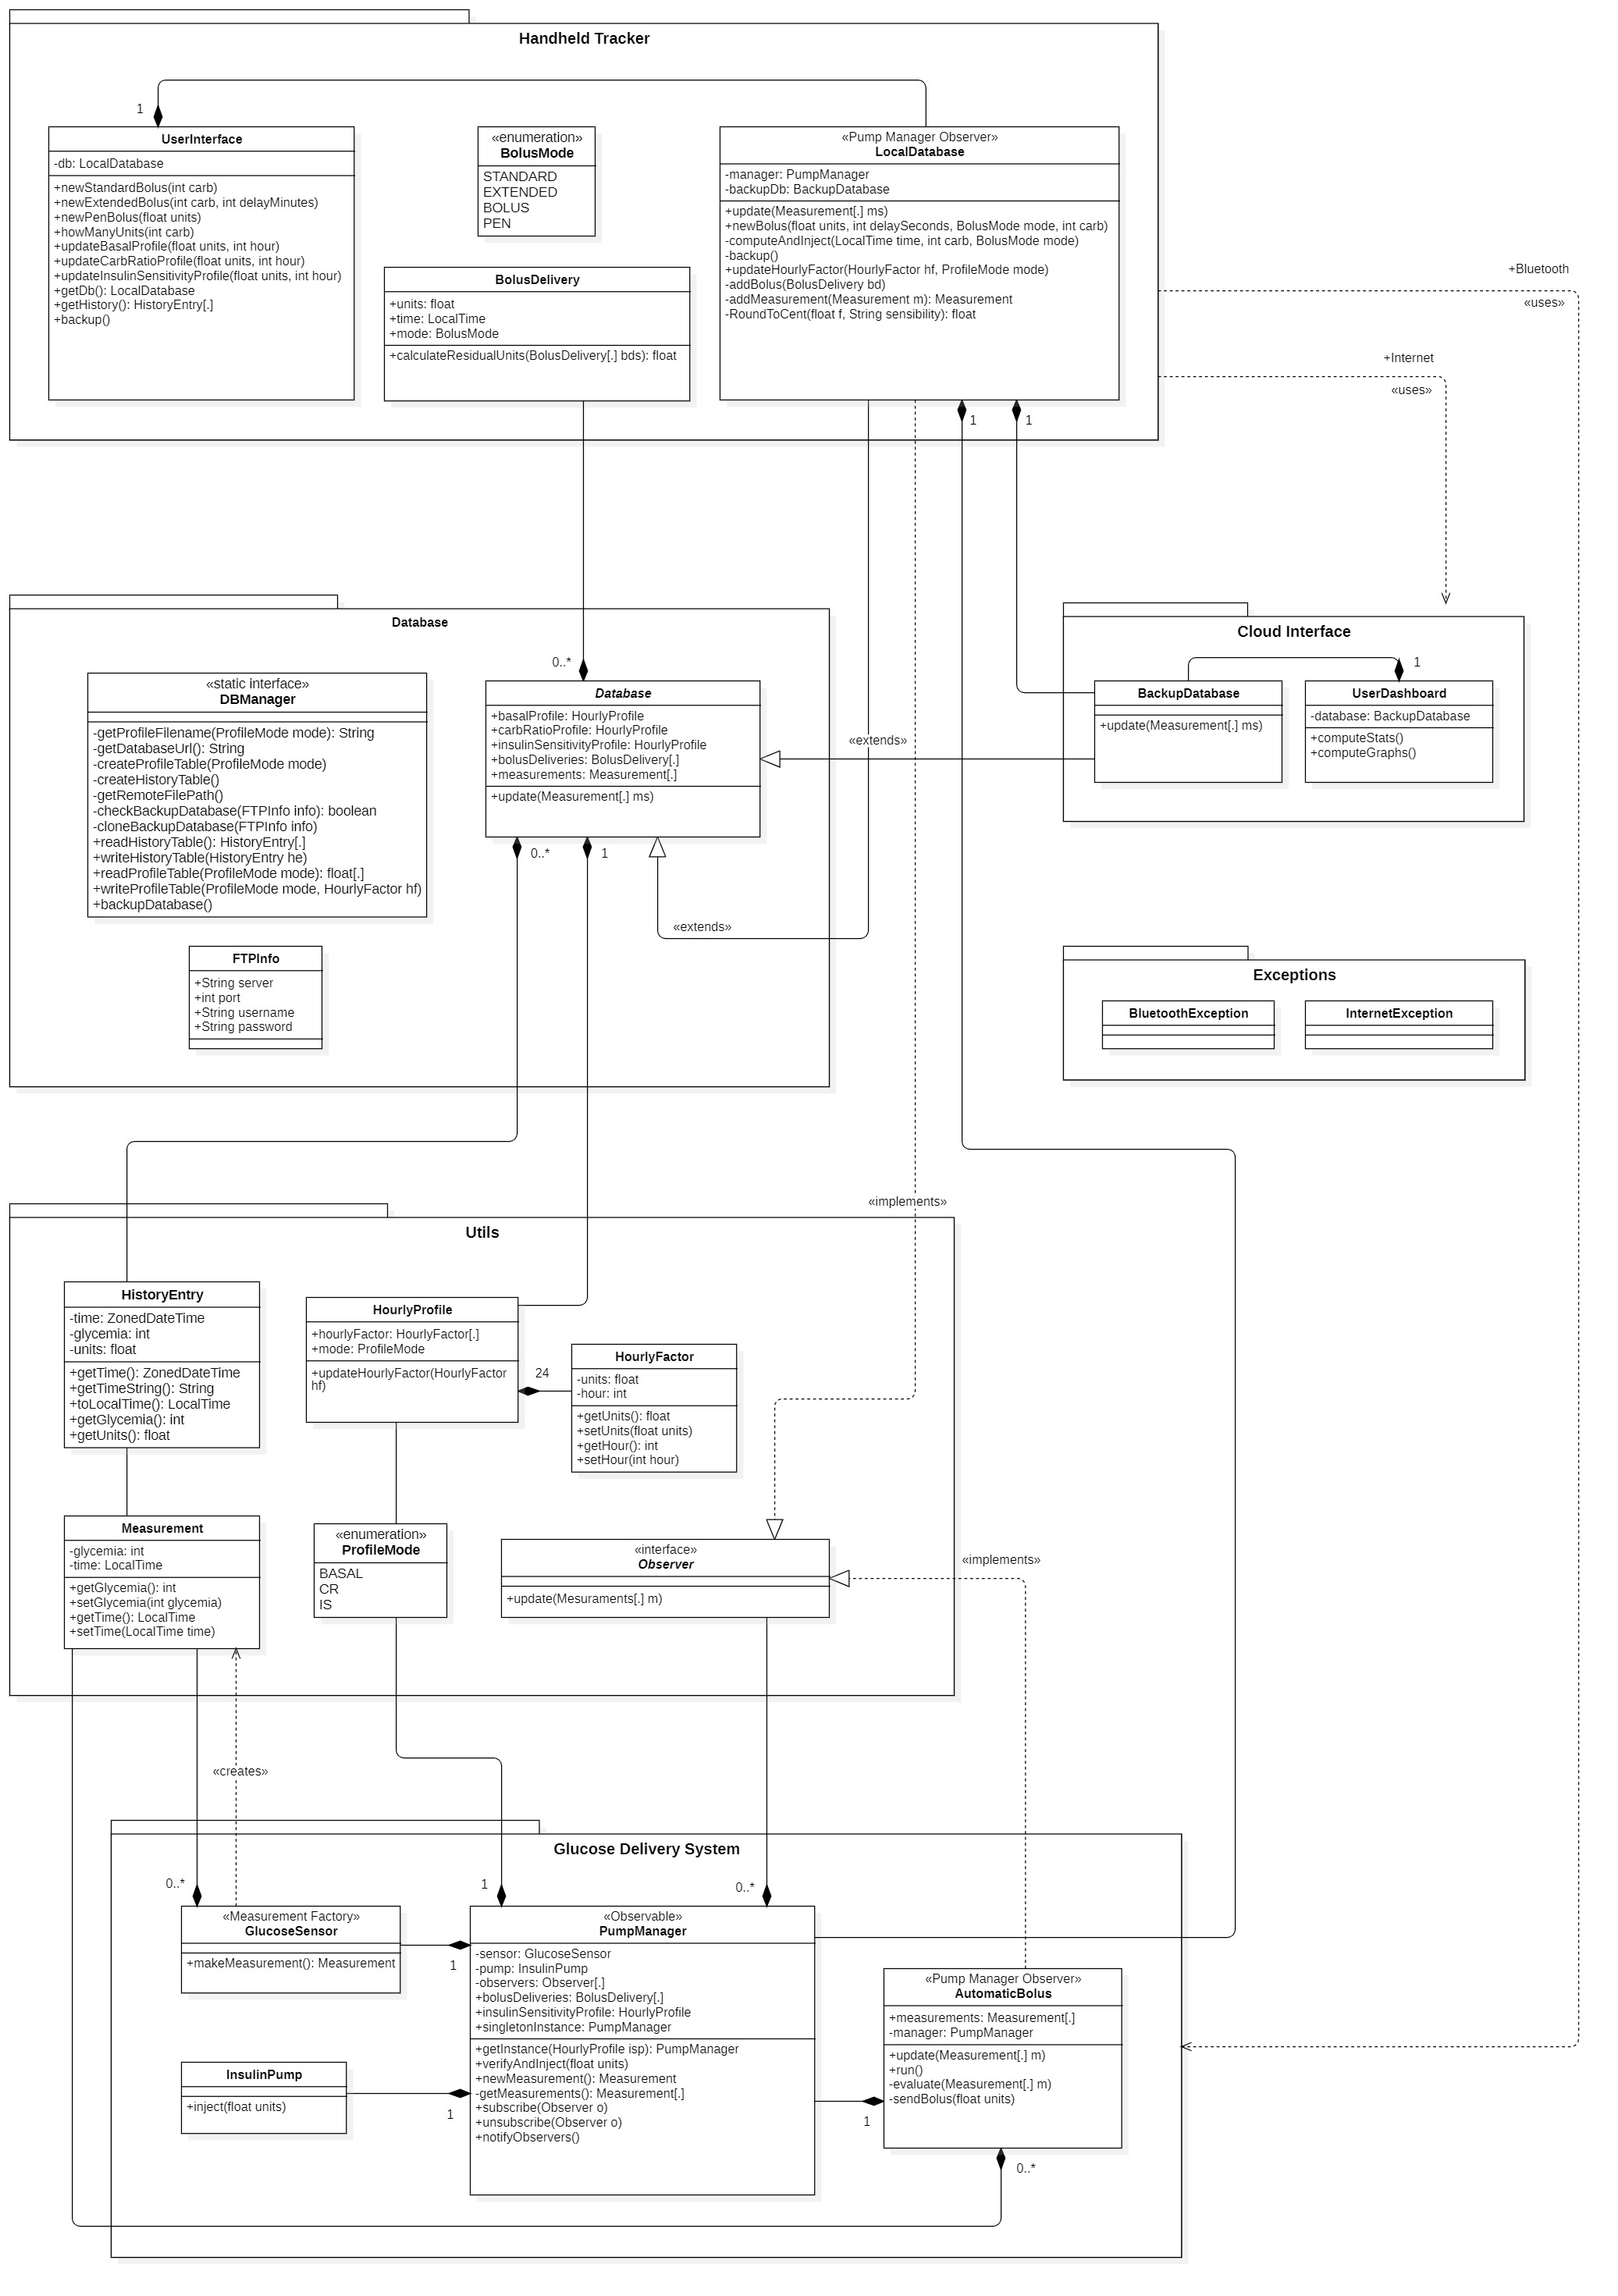
\includegraphics[width=16cm]{ClassDiagram.jpg}
    \caption{Class Diagram}
    \label{fig:class-diagram}
\end{figure}
\clearpage
\subsection{Classi ed Interfacce}

Per l’implementazione del nostro applicativo abbiamo sia definito nuove classi ed interfacce specifiche, sia utilizzato alcune di quelle già presenti nelle librerie standard di Java.

\subsubsection{Package Handheld Tracker}
è il package che rappresenta il palmare da cui comandare la pompa di insulina.

\textbf{User Interface}
\newline è l'interfaccia che con tutti i suoi metodi pubblici permette di eseguire tutto ciò che può richiedere l'utente: boli, aggiornamenti dei profili orari e backup.    
\begin{javaCode}{UserInterface.java}
public class UserInterface {
    private final LocalDatabase db;
    public UserInterface() { db = new LocalDatabase(); }
    public LocalDatabase getDb() { return db; }
    public HistoryEntry[] getHistory() { return DBManager.readHistoryTable(); }
    public void backup() { DBManager.backupDatabase(); }
    public void newStandardBolus(int carb) { db.newBolus(0, 0, BolusMode.STANDARD, carb); }
    public void newExtendedBolus(int carb, int delayMinutes) { // delay in minutes
        db.newBolus(0, delayMinutes * 60, BolusMode.EXTENDED, carb); // delay in seconds
    }
    public void howManyUnits(int carb) { db.newBolus(0, 0, BolusMode.MANUAL, carb); }
    public void newPenBolus(float units) { db.newBolus(units, 0, BolusMode.PEN, 0); }
    public void updateBasalProfile(float units, int hour) {
        db.updateHourlyFactor(new HourlyFactor(units, hour), ProfileMode.BASAL);
    }
    public void updateCarbRatioProfile(float units, int hour) {
        db.updateHourlyFactor(new HourlyFactor(units, hour), ProfileMode.CR);
    }
    public void updateInsulinSensitivityProfile(float units, int hour) {
        db.updateHourlyFactor(new HourlyFactor(units, hour), ProfileMode.IS);
    }
}
\end{javaCode}

\textbf{Local Database}
\newline è il centro nevralgico del sistema, estende la classe \texttt{Database} del package \texttt{Database} e si occupa di calcolare i boli raccogliendo le risorse necessarie, salva nel database i dati dei boli e dei profili di gestione e manda al \texttt{GlucoseDeliverySystem} (che rappresenta la pump) il calcolo delle unità di insulina da iniettare. Qui di seguito la funzione più importante di questa classe:
\begin{javaCode}{LocalDatabase.java - \textit{computeAndInject}}
try {
    // Get the last measurement if it exists
    if (measurements.isEmpty())
        manager.newMeasurement();

    Measurement lm = measurements.get(measurements.size() - 1);
    // Difference between last measurement and bolus time
    Duration diff = Duration.between(lm.getTime(), time);

    // Make a new measurement if the last one is older than 10 minutes from now
    if (diff.toMinutes() > 10) {
        manager.newMeasurement();
        lm = this.measurements.get(measurements.size() - 1);
    }
    // Get the actual hourly factors from profiles
    HourlyFactor sensitivity = insulinSensitivityProfile.hourlyFactors[LocalTime.now().getHour()];
    HourlyFactor carbRatio = carbRatioProfile.hourlyFactors[LocalTime.now().getHour()];

    // Create the BolusDelivery object
    BolusDelivery bd = new BolusDelivery(0, time, mode);

    // Compute the units of correction, units of carbohydrates and total units
    float glycUnits = 0;
    if (lm.getGlycemia() > 160)
        glycUnits = ((float) (lm.getGlycemia() - GLYC_REFERENCE)) / sensitivity.getUnits();
    float activeUnits = bd.calculateResidualUnits(bolusDeliveries);
    // Units of correction = Units of glycemia - Units of active insulin
    float correctionUnits = glycUnits - activeUnits;
    float carbUnits = 0;
    if (carb > 0 && carb <= 150)
        carbUnits = carb / carbRatio.getUnits();

    // Round the results to 2 decimal places
    bd.units = roundTo(correctionUnits + carbUnits, 0.01);
    glycUnits = roundTo(glycUnits, 0.01);
    activeUnits = roundTo(activeUnits, 0.01);
    correctionUnits = roundTo(correctionUnits, 0.01);
    carbUnits = roundTo(carbUnits, 0.01);

    if (bd.units > 0) {
        System.out.printf("%-16s%9s%14s%-18s%n", "Glycemia:", lm.getGlycemia() + " mg/dL", (glycUnits > 0 ? " " + glycUnits + " units" : ""), (correctionUnits != 0 ? "    correction" : ""));
        System.out.printf("%-25s%14s%-18s%n", "Active insulin:", (activeUnits > 0 ? "-" : "") + activeUnits + " units", "    " + (correctionUnits != 0 ? correctionUnits + " units" : ""));
        System.out.printf("%-16s%9s%14s%n", "Carbohydrates:", carb + " g    ", (carbUnits > 0 ? " " + carbUnits + " units" : ""));
        System.out.printf("%-25s%14s%n%n", "Total insulin:", (bd.units > 0 ? " " + bd.units + " units" : ""));

        boolean result = false;
        switch (mode) {
            case STANDARD:
                result = manager.verifyAndInject(bd.units);
                break;
            case EXTENDED:
                Duration delay = Duration.between(LocalTime.now(), time).plusSeconds(1); System.out.print("Waiting ");
                int hours = (int) delay.toHours();
                int minutes = (int) delay.toMinutes() % 60;
                int seconds = (int) delay.toSeconds() % 60;
                if (hours > 0)
                    System.out.print(hours + "h ");
                if (minutes > 0)
                    System.out.print(minutes + "m ");
                if (seconds > 0)
                    System.out.print(seconds + "s ");
                System.out.println("to inject " + bd.units + " units" + " at " + time.format(DateTimeFormatter.ofPattern("HH:mm")));
                Thread.sleep(delay.toMillis());

                result = manager.verifyAndInject(bd.units);

                break;
            case MANUAL:
                // Round the units to 0.5
                bd.units = roundTo(bd.units, 0.5);
                System.out.println("Manually inject: " + bd.units + " units");
            case PEN:
                result = true;
                break;
        }
        if (result) {
            DBManager.writeHistoryTable(new HistoryEntry(ZonedDateTime.now()lm.getGlycemia(), bd.units));
        } else {
            System.out.println("Injection failed");
        }
        addBolus(bd);
    } else if (bd.units == 0) {
        System.out.println("You don't need to inject insulin, you have a glycemia of: " + lm.getGlycemia() + " mg/dL");
    } else if (bd.units < 0) {
        System.out.println( "You don't need to inject insulin, you have " + activeUnits + " units of active insulin");
    }
} catch (Exception e) {
    e.printStackTrace();
    throw new BluetoothException();
}
\end{javaCode}


\textbf{Bolus Delivery}
\newline è la classe che ha come attributi \texttt{float units; LocalTime time; BolusMode mode} che permettono la rappresentazione di un oggetto bolo. Il suo unico metodo è \texttt{calculateResidualUnits} che prendendo in ingresso come parametro \texttt{List<BolusDelivery> bds} calcola attraverso una regressione linerare quante unità di insulina sono ancora attive. Qui di seguito la funzione più importante di questa classe:

\begin{javaCode}{BolusDelivery.java - calculateResidualUnits}
public float calculateResidualUnits(List<BolusDelivery> bds) {
    int hours = 3;
    float residualUnits = 0;
    if (!bds.isEmpty()) {
        // Cycle init
        int i = 0;
        // Init the last bolus
        BolusDelivery lb = bds.get(bds.size() - 1);
        Duration diff = Duration.between(lb.time, LocalTime.now());

        // While last bolus is not older than 3 hours
        while (diff.toMinutes() <= hours * 60 && i < bds.size()) {
            // Linear decay
            residualUnits += lb.units * (1 - (float) diff.toMinutes() / (hours * 60));
            // Cycle increment
            i++;
            // Last bolus
            lb = bds.get(bds.size() - i);
            // Difference between last bolus time and now
            diff = Duration.between(lb.time, LocalTime.now());
        }
    }
    return residualUnits;
}
\end{javaCode}


\textbf{Bolus Mode}
\newline rappresenta i 4 diversi tipi di bolo che possono esserci: \texttt{STANDARD, EXTENDED, MANUAL, PEN}.


\subsubsection{Package Database}

\textbf{DB Manager}
\newline si occupa della scrittura, lettura e backup del database e quindi del registro delle glicemie/boli, e dei tre \texttt{ProfileMode}: Basale, Rapporto Insulina Carboidrati e Rapporto Sensitività Insulinica.

\textbf{Database}
\newline ha come attributi: \texttt{HourlyProfile carbRatioProfile; HourlyProfile insulinSensitivityProfile; HourlyProfile basalProfile; List<BolusDelivery> bolusDeliveries; List<Measurement> measurements;} e fa da classe base per \texttt{LocalDatabase} e \texttt{BackupDatabase} che implementano il metodo \texttt{update}, che aggiunge alla lista dei Measurements le ultime misurazioni.

\textbf{FTP Info}
\newline ha come attributi: \texttt{String server; int port; String username; String password} che permettono di caricare il database su un server sqlite con le credenziale dettate da questa classe.


\subsubsection{Package Utils}

\textbf{History Entry}
\newline è il tipo base che ha come attributi glicemia, unità (d'insulina) e orario di somministrazione. Uno dei quattro registri nel database è composto da \texttt{HistoryEntry}. Come metodi sono implementati i getter e i setter.

\textbf{Measurement}
\newline è il tipo base che rappresenta una misurazione di glicemia (di cui il creatore è \texttt{glucoseDeliverySystem.GlucoseSensor}) e ha come attributi un intero corrispondente alla densità di glucosio nel sangue, misurata in $mg/dL$ e l'orario. Come metodi sono implementati i getter e i setter.

\textbf{Hourly Factor}
\newline è il tipo base che va a comporre tre dei quattro registri nel database: \texttt{BasalProfile}, \texttt{InsulineSensitivityProfile} e \texttt{CarbRatioProfile}. Ha come attributi delle unità e un orario (compreso tra $0$ e $23$, $24$ coincide con $0$) Come metodi sono implementati i getter e i setter.

\textbf{Hourly Profile}
\newline è composto da una lista di 24 \texttt{HourlyProfile} e da un attributo \texttt{ProfileMode mode}. Alla sua creazione se non è reperibile dal database la modalità corrispondente (attraverso il metodo \texttt{readProfileTable(mode)} della classe \texttt{DBManager} dal package \texttt{Database}), si andrà a creare un profilo di default. Qui di seguito la funzione più importante di questa classe che verifica che per ogni modalità i valori con cui aggiornare l'\texttt{HourlyFactor} siano in un certo range che permette sicurezza dell'utente:

\begin{javaCode}{HourlyProfile.java - updateHourlyFactor}
public void updateHourlyFactor(HourlyFactor hf) {
    boolean success = false;
    String modeString = "";
    if (hf.getHour() < 0 || hf.getHour() > 23)
        hf.setHour(hf.getHour());
    switch (mode) {
        case BASAL:
            modeString = "basal profile";
            if (hf.getUnits() >= 0.1 && hf.getUnits() <= 5)
                success = true;
            break;
        case CR:
            modeString = "carb ratio";
            if (hf.getUnits() >= 1 && hf.getUnits() <= 15)
                success = true;
            break;
        case IS:
            modeString = "insulin sensitivity";
            if (hf.getUnits() >= 20 && hf.getUnits() <= 50)
                success = true;
            break;
    }
    if (success) {
        System.out.println("Updating " + modeString + " h=" + hf.getHour() + " from " + String.format("%.2f", hourlyFactors[hf.getHour()].getUnits()).replace(",", ".") + " to " + String.format("%.2f", hf.getUnits()).replace(",", ".") + "...");
        hourlyFactors[hf.getHour()] = hf;
    } else {
        System.out.println("Invalid " + modeString + " value");
    }
}
\end{javaCode}

\textbf{Profile Mode}
\newline rappresenta i 3 diversi tipi di HourlyProfile che possono esserci: \texttt{BASAL, CR, IS} corrispondenti rispettivamente ai profili di Basale, Rapporto insulina carboidrati e Rapporto Sensitività insulinica.

\textbf{Observer}
\newline interfaccia per il design pattern Observer implementato poi nel \texttt{handheldTracker.LocalDatabase}.


\subsubsection{Package Glucose Delivery System}

\textbf{Pump Manager}
\newline gestore principale del \texttt{GlucoseDeliverySystem}. Implementa i design pattern Observer, chiama il Factory e la creazione della sua istanza è un Singleton (esisterà solo un oggetto \texttt{PumpManager}). Permette di mandare le informazioni all'\texttt{InsulinPump} tramite il metodo:
\begin{javaCode} {PumpManager.java - verifyAndInject}
public boolean verifyAndInject(float units) {
    if (units > 0 && units <= 20) {
        bds.add(new BolusDelivery(units, LocalTime.now(), BolusMode.STANDARD));
        pump.inject(units);
        return true;
    } else if (units > 20) {
        System.out.println("Too many units");
    } else {
        System.out.println("Invalid units");
    }
    return false;
}
\end{javaCode}
permette di chiamare una nuova misurazione e dunque la chiamata della factory \texttt{GlucoseSensor} tramite il metodo:
\begin{javaCode} {PumpManager.java - verifyAndInject}
public Measurement newMeasurement() {
    Measurement m = sensor.makeMeasurement();
    this.measurements.add(m);

    notifyObservers();
    return m;
}
\end{javaCode}

\textbf{Glucose Sensor}
\newline crea un oggetto \texttt{Measurement} e di fatto implementa il desing pattern Factory.

\textbf{Insulin Pump}
\newline inietta il quantitativo di insulina che riceve dal \texttt{PumpManager} e stampa il risultato.

\textbf{Automatic Bolus}
\newline fornisce una routine che ogni $10$ o $15$ minuti inietta rispettivamente \(\frac{1}{6}\) o \(\frac{1}{4}\) della basale relativa all'orario corrente, a cui è sommata una correzione per far tornare la glicemia in un range corretto, indicativamente di $80-150$ (non è sommata se la glicemia è già nel range), e manda il tutto al \textttt{PumpManager}.


\subsubsection{Package Cloud Interface}

\textbf{Backup Database}
\newline tiene traccia del backup del database quando invocato.

\textbf{User Dashboard}
\newline fornisce statistiche e grafici dei dati presenti nella History.


\subsubsection{Package Exceptions}

\textbf{Bluetooth Exception}
\newline classe che rappresenta l'eccezione se non riesce il collegamento tra l'Handheld Tracker e il Glucose Delivery System.

\textbf{Internet Exception}
\newline  classe che rappresenta l'eccezione se non riesce il collegamento tra l'Handheld Tracker e la Cloud Interface.


\subsection{Design Patterns}
All’interno del progetto abbiamo avuto la necessità di introdurre alcuni design patterns noti per favorire la gestione di alcune dipendenze tra classi in modo agile ed elegante. I patterns utilizzati sono:
\begin{itemize}
    \setlength\itemsep{0em}
    \item \textbf{Observer}
    \item \textbf{Singleton}
    \item \textbf{Factory}
\end{itemize}

\subsubsection{Observer}
\begin{javaCode}{Implementazione di Observer - handheldTracker.LocalDatabase.java}
public class LocalDatabase extends Database implements Observer {
    // ...
    @Override
    public void update(List<Measurement> ms) {
        super.update(ms);
        backup();
    }
}

class Database {
    public List<Measurement> measurements;

    protected void update(List<Measurement> ms) {
        for (Measurement m : ms) {
            measurements.add(m);
        }
    }
}
\end{javaCode}
\begin{javaCode}{Implementazione di Observable - glucoseDeliverySystem.PumpManager}
public class PumpManager {
    private List<Measurement> measurements = new ArrayList<>();
    private final List<Observer> observers = new ArrayList<>();
    // ...
    public void subscribe(Observer o) { observers.add(o); }
    
    public void unsubscribe(Observer o) { observers.remove(o); }
    
    private void notifyObservers() {
        for (Observer observer : observers) {
            observer.update(this.measurements);
        }
    }
}
\end{javaCode}

\newpage
\subsubsection{Singleton}
\begin{javaCode}{Implementazione di Singleton - glucoseDeliverySystem.PumpManager}
public class PumpManager {
    // ...
    private static PumpManager SingletonInstance;

    private PumpManager(HourlyProfile isp) { ... }

    public static PumpManager getInstance(HourlyProfile isp) {
        if (SingletonInstance == null) {
            SingletonInstance = new PumpManager(isp);
        } else {
            SingletonInstance.insulinSensitivityProfile = isp;
        }
        return SingletonInstance;
    }
}
\end{javaCode}

\subsubsection{Factory}
\begin{javaCode}{Implementazione di Factory - glucoseDeliverySystem.GlucoseSensor}
public class GlucoseSensor {
    public Measurement makeMeasurement() {
        int min = 60;
        int max = 300;
        int glycemia = (int) Math.abs(Math.random() * (max - min) + min);
        return new Measurement(glycemia, LocalTime.now());
    }
}
\end{javaCode}

\subsection{Disposizione delle classi nei vari package}

\vspace{1.5em}
\begin{figure}[H]
    \centering
    \captionsetup{justification=centering,margin=2cm}
    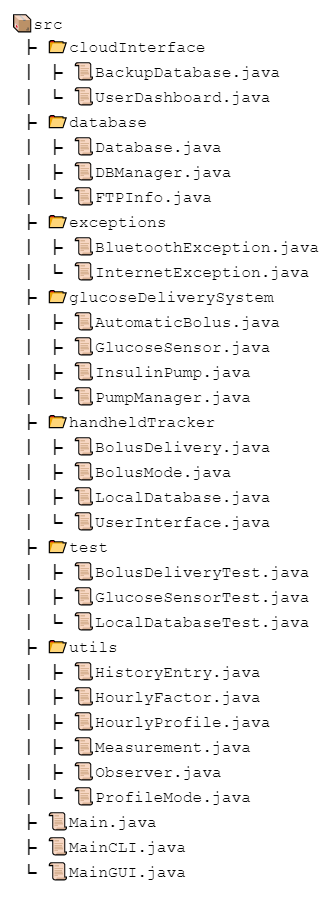
\includegraphics{FileTree.png}
    \caption{Raffigurazione della disposizione delle classi del progetto nei package}
    \label{fig:packages}
\end{figure}

\newpage

\section{Unit Test}

Per testare la corretta interazione e collaborazione fra le parti abbiamo realizzato i seguenti test cases per alcune delle classi principali dell’applicativo:
Nel progetto è stato utilizzato il framework \href{https://junit.org/junit5/}{\textit{JUnit 5}}.
In tutte e tre le classi di test faremo uso di
\begin{javaCode} {Import necessari per il testing}
import org.junit.Test;
import static org.junit.Assert.*;
\end{javaCode}
L'import statico permette di chiamare direttamente il metodo \texttt{assertEquals(expected,actual,delta)} che fa fallire il test se

\[expected \neq actual \pm delta\]

È possibile trovare tutta la parte di codice riguardante all'unit testing nella cartella \href{https://github.com/federicomarra/swe-diab/tree/master/src/test}{\textit{src/test}}

\subsection{Bolus Delivery Test}
In questa suite di test viene controllato che gli oggetti creati appartenenti alla classe \texttt{BolusDelivery} 

\subsubsection{Constructor Test}
Il metodo \texttt{ConstructorTest} nella classe \texttt{BolusDeliveryTest} è un test unitario che verifica che avvenga correttamente la creazione dell'oggetto \texttt{BolusDelivery} in tutte e 4 le modalità: standard, esteso, manuale e con penna. Inizialmente viene casualmente deciso un certo numero di unità in un range tra 1 e 15 con uno scalino di 0.01 per le prime due modalità, e con lo scalino di 0.5 per le restanti modalità; viene ulteriormente creato anche un \texttt{delay} tra 1 e 15 minuti. Si crea l'oggetto con come parametri passati in ingresso al costruttore i valori creati precedentemente, in seguito si testa che gli attributi dell'oggetto corrispondano a quelli che con cui è stato creato l'oggetto: \texttt{units} e orario testando ora, minuti e secondi dell'attributo \texttt{time}. Tutto ciò viene fatto per tutte e quattro le modalità.

\subsubsection{Calculate Residual Units Test}
Il metodo \texttt{calculateResidualUnitsTest} nella classe \texttt{BolusDeliveryTest} è un test unitario che verifica il corretto funzionamento del metodo \texttt{calculateResidualUnits} della classe \texttt{BolusDelivery}. Inizializza alcune variabili, genera un oggetto \texttt{BolusDelivery} con attributi casuali, e successivamente esegue due test:
\begin{enumerate}
    \item Il primo test verifica che venga restituito $0$ quando chiamato su una lista vuota di oggetti \texttt{BolusDelivery}.
    \item Il secondo test aggiunge l'oggetto \texttt{BolusDelivery} generato a una lista e verifica che il metodo restituisca un valore specifico, calcolato in base agli attributi dell'oggetto e agli elementi nella lista.
\end{enumerate}


\subsection{Glucose Sensor Test}
In questa suite di test viene controllato che gli oggetti creati appartenenti alla classe \texttt{GlucoseSensor} 

\subsubsection{Constructor Test}
Il metodo \texttt{ConstructorTest} nella classe \texttt{GlucoseSensorTest} è un test unitario che verifica il corretto funzionamento del metodo \texttt{newMeasurement} della classe \texttt{PumpManager}. In breve, il test crea un'istanza di \texttt{PumpManager} con un profilo orario, chiama il metodo \texttt{newMeasurement} per generare una nuova misurazione della glicemia, la memorizza in una variabile e verifica che questa misurazione sia correttamente aggiunta alla lista interna di misurazioni. Se l'asserzione passa, il test conferma che il metodo \texttt{newMeasurement} funziona come previsto; altrimenti, indica la presenza di un bug che richiede correzione.


\subsection{Local Database Test}
In questa suite di test viene controllato che gli oggetti creati appartenenti alla classe \texttt{LocalDatabase}

\subsubsection{Constructor Test}
 nella classe \texttt{LocalDatabaseTest} è un test unitario che verifica il corretto funzionamento del costruttore nella classe \texttt{LocalDatabase}. Ecco una spiegazione passo dopo passo di come funziona:
\begin{enumerate}
    \item Innanzitutto, crea un'istanza di \texttt{LocalDatabase} chiamando il suo costruttore.
    \item Successivamente, verifica tramite un'asserzione che la lista \texttt{bolusDeliveries} nell'istanza di \texttt{LocalDatabase} sia vuota. Ciò verifica che il costruttore inizializzi correttamente la lista \texttt{bolusDeliveries}.
    \item Verifica anche tramite un'asserzione che la lista \texttt{measurements} nell'istanza di \texttt{LocalDatabase} sia vuota. Ciò verifica che il costruttore inizializzi correttamente la lista \texttt{measurements}.
    \item Verifica tramite un'asserzione che l'array \texttt{hourlyFactors} nei profili \texttt{carbRatioProfile}, \texttt{insulinSensitivityProfile} e \texttt{basalProfile} dell'istanza di \texttt{LocalDatabase} abbia ciascuno una lunghezza di 24. Ciò verifica che il costruttore inizializzi correttamente questi profili con 24 fattori orari.
\end{enumerate}
Se tutte le asserzioni passano, significa che il costruttore nella classe \texttt{LocalDatabase} sta funzionando come previsto. Se una qualsiasi asserzione fallisce, l'intero test fallisce.

\subsubsection{New Bolus Test}
Il test \texttt{newBolusTest} nella classe \texttt{LocalDatabaseTest} verifica il corretto funzionamento del metodo \texttt{newBolus} nella classe \texttt{LocalDatabase}. Durante il test, viene creata un'istanza di \texttt{LocalDatabase}, generato un valore casuale rappresentante le unità di insulina, creato un oggetto \texttt{BolusDelivery} con questo valore e altre informazioni, chiamato il metodo \texttt{newBolus}, e infine verificato che la lista di somministrazioni \texttt{bolusDeliveries} sia stata aggiornata correttamente con l'aggiunta di questo nuovo oggetto \texttt{BolusDelivery}. Se tutte le verifiche passano, il test conferma che il metodo \texttt{newBolus} funziona come previsto; in caso contrario, il test fallisce.

\subsubsection{Compute And Inject Test}
Il test \texttt{computeAndInjectTest} nella classe \texttt{LocalDatabaseTest} verifica il corretto funzionamento del metodo \texttt{computeAndInject} della classe \texttt{LocalDatabase}, indirettamente attraverso il metodo \texttt{newBolus}. Di seguito una spiegazione in breve del funzionamento:
\begin{enumerate}
    \item Viene creata un'istanza di \texttt{LocalDatabase} chiamata \texttt{db}.
    \item Si generano valori casuali per i carboidrati \texttt{c} e la glicemia \texttt{g}.
    \item Viene aggiunto un nuovo oggetto \texttt{Measurement} alla lista \texttt{measurements} in \texttt{db} rappresentando una misurazione della glicemia.
    \item Vengono recuperati i fattori orari per la sensibilità ai carboidrati \texttt{csens} e la sensibilità all'insulina \texttt{isens} da \texttt{db}.
    \item Si calcolano le unità attese \texttt{u} di insulina considerando i fattori orari e la presenza di correzione.
    \item Si randomizza la modalità del bolo \texttt{mode} e, se applicabile, il ritardo.
    \item Viene creato un oggetto \texttt{BolusDelivery} con le informazioni calcolate.
    \item Si chiama il metodo \texttt{newBolus} con le informazioni dell'oggetto \texttt{BolusDelivery}, il quale a sua volta richiama internamente \texttt{computeAndInject}.
    \item Dopo la chiamata, il test verifica che la lista \texttt{bolusDeliveries} in \texttt{db} sia stata aggiornata correttamente, confrontando l'ultima voce con l'oggetto \texttt{BolusDelivery} creato.
    \item Vengono verificati unità, orario e modalità dell'ultimo \texttt{BolusDelivery} nella lista. Se tutti questi valori corrispondono a quelli dell'oggetto \texttt{BolusDelivery}, il test è superato.
\end{enumerate}

\subsubsection{Update Hourly Factor Test}
Il test \texttt{updateHourlyFactorTest} è un test unitario nella classe \texttt{LocalDatabaseTest} che verifica il corretto funzionamento del metodo \texttt{updateHourlyFactor} della classe \texttt{LocalDatabase}. Ecco una spiegazione dettagliata di come funziona:
\begin{enumerate}
    \item Inizialmente, crea un'istanza di \texttt{LocalDatabase} denominata \texttt{db}.
    \item Successivamente, inizializza due array \texttt{hours} e \texttt{units} di dimensione 3. L'array \texttt{hours} conterrà ore casuali tra 0 e 23, mentre l'array \texttt{units} conterrà unità casuali di insulina.
    \item Il test esegue quindi tre sub-test, uno per ciascuna modalità di profilo: \texttt{BASAL}, \texttt{CR} (Rapporto Carboidrati), e \texttt{IS} (Sensibilità Insulinica).
    \item Per il test del profilo \texttt{BASAL}, genera un numero casuale in virgola mobile \texttt{units[0]} tra 0.01 e 5 con una precisione di 0.05. Crea un oggetto \texttt{HourlyFactor} chiamato \texttt{hf0} con \texttt{units[0]} e un'ora casuale \texttt{hours[0]}. Successivamente, chiama il metodo \texttt{updateHourlyFactor} dell'istanza di \texttt{LocalDatabase} chiamata \texttt{db} con \texttt{hf0} e \texttt{ProfileMode.BASAL}. Dopo la chiamata del metodo, il test verifica se l'array list \texttt{hourlyFactors} nel profilo \texttt{basalProfile} dell'istanza di \texttt{LocalDatabase} \texttt{db} è stato aggiornato correttamente. Fa ciò verificando tramite un'asserzione che l'ora e le unità dell'\texttt{HourlyFactor} all'indice \texttt{hours[0]} corrispondano all'ora e alle unità di \texttt{hf0}.
    \item Per il test del profilo \texttt{CR}, genera un numero intero casuale \texttt{units[1]} tra 1 e 15. Crea un oggetto \texttt{HourlyFactor} chiamato \texttt{hf1} con \texttt{units[1]} e un'ora casuale \texttt{hours[1]}. Successivamente, chiama il metodo \texttt{updateHourlyFactor} dell'istanza di \texttt{LocalDatabase} \texttt{db} con \texttt{hf1} e \texttt{ProfileMode.CR}. Dopo la chiamata del metodo, il test verifica se l'array list \texttt{hourlyFactors} nel profilo \texttt{carbRatioProfile} dell'istanza di \texttt{LocalDatabase} \texttt{db} è stato aggiornato correttamente. Fa ciò verificando tramite un'asserzione che l'ora e le unità dell'\texttt{HourlyFactor} all'indice \texttt{hours[1]} corrispondano all'ora e alle unità di \texttt{hf1}.
    \item Per il test del profilo \texttt{IS}, genera un numero intero casuale \texttt{units[2]} tra 20 e 50. Crea un oggetto \texttt{HourlyFactor} chiamato \texttt{hf2} con \texttt{units[2]} e un'ora casuale \texttt{hours[2]}. Successivamente, chiama il metodo \texttt{updateHourlyFactor} dell'istanza di \texttt{LocalDatabase} \texttt{db} con \texttt{hf2} e \texttt{ProfileMode.IS}. Dopo la chiamata del metodo, il test verifica se l'array list \texttt{hourlyFactors} nel profilo \texttt{insulinSensitivityProfile} dell'istanza di \texttt{LocalDatabase} \texttt{db} è stato aggiornato correttamente. Fa ciò verificando tramite un'asserzione che l'ora e le unità dell'\texttt{HourlyFactor} all'indice \texttt{hours[2]} corrispondano all'ora e alle unità di \texttt{hf2}.
\end{enumerate}

\newpage


\section{Integrazione Continua}

Per rilasciare automaticamente il pacchetto GUI abbiamo sviluppato un \href{https://docs.github.com/en/actions/using-workflows}{\textit{Workflow Github}} che esegue lo script Maven di build e successivamente crea una \href{https://docs.github.com/en/repositories/releasing-projects-on-github/managing-releases-in-a-repository}{\textit{Release Github}} contenente il file \texttt{.jar} aggiornato.

Questo workflow viene eseguito ogni volta che il codice è modificato sulla repository pubblica, cioè quando viene fatto un nuovo commit o pull request sul branch principale oppure manualmente tramite l'UI di Github cliccando il \href{https://docs.github.com/en/actions/using-workflows/manually-running-a-workflow}{\textit{bottone relativo a questa azione}}.

\vspace{2.4em}
\begin{figure}[!htbp]
    \centering
    \begin{yamlCode}{maven.yml}
steps:
  - uses: actions/checkout@v3

  - name: "Set up JDK 11"
    uses: actions/setup-java@v3
    with:
      java-version: "11"
      cache: maven

  - name: "Build with maven"
    run: mvn clean -B package --file pom.xml

  - name: "Set up git"
    run: git config --global user.email "github-actions@github.com" && git config --global user.name "GitHub Actions"

  - name: "Change file name"
    run: mv ./target/swe-diab-1.0.0-jar-with-dependencies.jar ./target/swe-diab.jar

  - name: "Delete previous release"
    run: gh release delete v1.0.0 --yes

  - name: "Create new release"
    run: gh release create v1.0.0 ./target/swe-diab.jar -t "v1.0.0" -n "Version 1.0.0"

  - name: "Upload executable as release asset"
    run: gh release upload v1.0.0 ./target/swe-diab.jar --clobber
\end{yamlCode}

\end{figure}


% LIST OF FIGURES AND TABLES %

\newpage

\listoffigures      % Lista delle figure

\listoftables       % Lista delle tabelle

\end{document}